% !TeX root = ../../thesis.tex
\chapter{Introduction}\label{ch:introduction}

This chapter provides an overview of non-valence anions in general and particularly dipole bound anions. The current research that has viewd the presence of both dbas and biological systems is presented. it then presents the system of interest, biological quinoones, and their role in biological process. Ffinally the research goals are especified.

\section{Nonvalence Anions}
Anions are molecules with an excess electron. Anions generally require specific care in terms of their ab initio description because of the more diffuse nature of the valence
orbitals \cite{simons2008molecular,simons2023molecular}. The first conception of the NBS was given in 1947 by Fermi and Teller, who predicted that an excess electron could be held by a non-rotating dipole field of a neutral core if its dipole moment exceeds 1.625 D \cite{fermi1947capture}.
Nonvalence anions (NBS) \newglossaryentry{NBS}{name={NBS},description={Non-Valence Anion}} represent a class of molecular anions where the extra electron occupies a diffuse orbital that is spatially decoupled from the usual valence orbitals of the molecule.\cite{jordan2003theory}. These have been studied extensively by spectroscopic means in the gas phase in the last years, they have weaken a lot of interest \cite{kang2024reaction}.
Solvated electrons could be considered a nonvalence statre, although still a debated topic, the main theory and observations point to the electron residing in a cavity of 2.5 \r{A} \cite{herbert2017hydrated}.

\subsection{Dipole Bound Anions}
When it comes to the theoretical study of DB anions, twochallenges are faced. First, one must use atomic orbital basisfunctions that are sufficiently diffuse to describe the spatialextent of the DB orbital, usually this means using custom basis sets \cite{skurski2000choose}.
Although the electron boundwithin the DB orbital resides to a large extent far away from theprecursor's valence electrons, it still has a significantly largedispersion-like interaction with the latter electrons to contributesubstantially to the EBE. That is, the DB orbital is quitepolarizable, so it would be expected to have a substantial van derWaals (i.e., dispersion) interaction with other nearby electrondensities\cite{gutowski1996contribution}
Apart from the esoteric nature of their studies as theoretical objects and in carefuly prepared experiments, dipole bound anions are of great interest due to their presence in various fields, including astrchemistry \cite{fortenberry2015interstellar}, and radiation biology\cite{narayanan2023secondary,sedmidubska2024interaction}. The main interest for them is when the parent molecule also supports a valence anion state. In this case, the DBA can act as a doorway state electrons for the more stable VBA.

When solvent molecules are considered, becaptured by nearby solvent molecules which have undergonereorientation to form a solvation cage around the electron, or (c)be captured by nearby solvent molecules whose instantaneousdipole orientations happen to be favorable to forming a DB state.The latter two cases arise is so-called charge-transfer-to-solvent(CTTS) electronic transitions \cite{bradforth2002excited,chen2000precursors}.

\section{Dipole Bound Anions in Biology}
The bast majority of research on dipole bound anions has been conducted in gas phase. Related to biological research, the most relevant work has been done on the interaction of dipole bound anions with DNA. The main focus of these studies has been on the radiation damage to DNA \cite{narayanan2023secondary} and the role of dipole bound anions as radiosensitizers \cite{sedmidubska2024interaction}. \\
The existance of NBS in condensed matter is still debated. For instance, A QM study of the effects of hydration on the DB state of a model polar species showed that the excess electron migrates into an orbital localized on the outer surface of the water solvent cage \cite{anusiewicz2020fate}. However, it has been experimentaly shown that a DBS is not destroyed by the presence of an alkyl chain \cite{castellani2019stability}. Another study found that a DBS mediated doorway mechanism exists in both microsolvated and bulk-solvated uracil-DEG systems \cite{narayanan2024electron} Ths leads to the questions of can the NBS survive in the bulk? In an apolar solvent, the density of molecules is too large and the excluded volume will not allow a DBS to exist. In polar solvents, the solvent itself can provide a dipolar stabilisation as is the case for charge-transfer-to-solvent (CTTS) states,\cite{bradforth2002excited,chen2000precursors} which may be viewed as a DBS. However, much of biology exists as softmatter, for which the molecular density can be much lower. For example, proteins contain large vacant pockets, which
could accommodate a DBS that may have small molecular
fragments poking into it.

Little work has been done to assess their role in natural pathways. It is possible that they could provide an elegant way to regulate long-range electron transfer. Due to their strong dependence on to the surroundings, they could provide.Uracil water \cite{clarke2025role}.
This has been limited by the expensive methods needed to study these states, only allowing to study small systems.\\
\subsection{Experimental Studies overview}
\subsection{overlap with biochemical systems}
Interactions of electrons with bare and hydrated biomolecules: From nucleic acid bases to DNA segments \cite{gu2012interactions}. 
It has been sugested that the dipole bound anions could be importnat in the cases of flavines \cite{matthews2018observation}

\section{Biological quinones}
To trace this history from its source we must go back to 1785, when an apothecary of the name of Hofmann obtained the calcium salt of an acid called quinic acid from Cinchona bark. This acid is now known to be of common occurrence in plants ; it exists in the bilberry and in coffee, in holly, ivy, oak, elm, and ash leaves, and probably many other leaves. Liebig also prepared the calcium salt, and was the first to give a complete analysis... he proposed in place of it the name quinone, by which it is still known
The origin of the name “quinone” itself is interesting. It comes from quinic acid, as quinone was first obtained in the oxidation reaction of this acid, which at its time is obtained from the bark of cinchona and the word ending -one comes from the ketone group (ketone)\cite{chen2024low,rusell1873quinone}. 
The role of ubiquinones in biological processes cannot be overestimated...\cite{ernster1995biochemical}.
Quinones are a class of molecules that are ubiquitous in biological systems. Quinones act as electron carriers between different enzymes, facilitating the transfer of electrons and protons in redox reactions. It is generally accepted
that the isoprenoid side chain of the coenzyme takes part in intermolecular interactions. The mitochondrial Complex I has
an L-shaped structure. Electrons produced by NADH oxidation are
transported along the hydrophilic arm through a series of Fe-S
clusters. The second arm, embedded in the mitochondrial inner
membrane, provides an amphipathic environment composed of
charged and hydrophobic ends. The ubiquinone chamber stretches
through the boundary between the two arms, and recently
reported free energy profiles unveiled the interplay between the
interactions of the ubiquinone head and tail. Electron transfer
takes place as the CoQ 0 head approaches the closest lying cluster,
labelled N2, while diffusion of the isoprenoid tail along the mitochondrial inner membrane carries the electrons to the subsequent
stages of aerobic cell respiration. The CoQ 0 head can form hydrogen
bonds with water molecules (micro-hydration) and nearby amino
acid residues in the hydrophilic arm, while the tail is responsible for hydrophobic interactions in the membrane, although with some degree of hydration.

Coenzyme Q (ubiquinone) is one of the most common quinones found in nature, and its structure allows for the stabilization of both valence and dipole-bound anionic states. This unique property makes quinones an interesting subject for studying the potential existence and role of nonvalence anions in biological systems.

The dipole bound anion in 2-3-dimethoxy-para-benzoquinone (CoQ0), has been observed experimentaly \cite{ameixa2023parent,west2014anion,pshenichnyuk2020ionizing, bull2015anion}. for CoQ1 it is still seen but much weaker, and for CoQ2 it is not. 

\section{Research Goals}

% Some dummy code show how to include images.
\begin{figure}[th!]
  \centering
  \medskip
  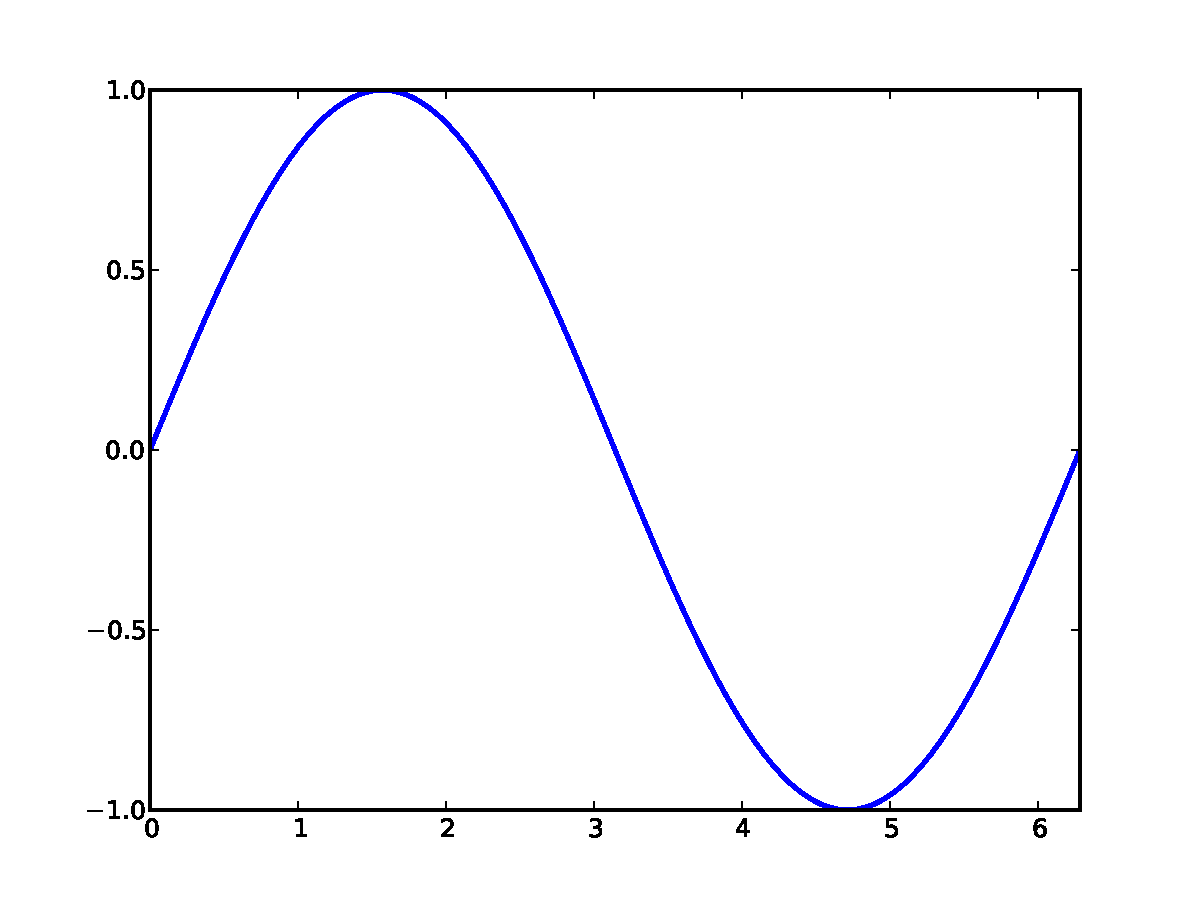
\includegraphics[width=.9\textwidth]{sine}
  \caption[Short caption for Table of Figures]{Illustration of how to
  include a figure (long text, should not go to Table of Figures).}
  \label{fig:sine}
\end{figure}

%Add list of symbols and abbreiations here:
% Some dummy code to get at least 1 entry in the nomenclature.
\nomenclature{$\Theta$}{A nice symbol}
Introducing some symbol: $\Theta$.

% Some dummy code to get at least 1 entry in the list of
% abbreviations.
\newglossaryentry{md}{name={MD},description={molecular dynamics}}
Introducing an acronym: \gls{md}.

\begin{figure}[th!]
  \centering
  % GNUPLOT: LaTeX picture with Postscript
\begingroup
  \makeatletter
  \providecommand\color[2][]{%
    \GenericError{(gnuplot) \space\space\space\@spaces}{%
      Package color not loaded in conjunction with
      terminal option `colourtext'%
    }{See the gnuplot documentation for explanation.%
    }{Either use 'blacktext' in gnuplot or load the package
      color.sty in LaTeX.}%
    \renewcommand\color[2][]{}%
  }%
  \providecommand\includegraphics[2][]{%
    \GenericError{(gnuplot) \space\space\space\@spaces}{%
      Package graphicx or graphics not loaded%
    }{See the gnuplot documentation for explanation.%
    }{The gnuplot epslatex terminal needs graphicx.sty or graphics.sty.}%
    \renewcommand\includegraphics[2][]{}%
  }%
  \providecommand\rotatebox[2]{#2}%
  \@ifundefined{ifGPcolor}{%
    \newif\ifGPcolor
    \GPcolortrue
  }{}%
  \@ifundefined{ifGPblacktext}{%
    \newif\ifGPblacktext
    \GPblacktexttrue
  }{}%
  % define a \g@addto@macro without @ in the name:
  \let\gplgaddtomacro\g@addto@macro
  % define empty templates for all commands taking text:
  \gdef\gplbacktext{}%
  \gdef\gplfronttext{}%
  \makeatother
  \ifGPblacktext
    % no textcolor at all
    \def\colorrgb#1{}%
    \def\colorgray#1{}%
  \else
    % gray or color?
    \ifGPcolor
      \def\colorrgb#1{\color[rgb]{#1}}%
      \def\colorgray#1{\color[gray]{#1}}%
      \expandafter\def\csname LTw\endcsname{\color{white}}%
      \expandafter\def\csname LTb\endcsname{\color{black}}%
      \expandafter\def\csname LTa\endcsname{\color{black}}%
      \expandafter\def\csname LT0\endcsname{\color[rgb]{1,0,0}}%
      \expandafter\def\csname LT1\endcsname{\color[rgb]{0,1,0}}%
      \expandafter\def\csname LT2\endcsname{\color[rgb]{0,0,1}}%
      \expandafter\def\csname LT3\endcsname{\color[rgb]{1,0,1}}%
      \expandafter\def\csname LT4\endcsname{\color[rgb]{0,1,1}}%
      \expandafter\def\csname LT5\endcsname{\color[rgb]{1,1,0}}%
      \expandafter\def\csname LT6\endcsname{\color[rgb]{0,0,0}}%
      \expandafter\def\csname LT7\endcsname{\color[rgb]{1,0.3,0}}%
      \expandafter\def\csname LT8\endcsname{\color[rgb]{0.5,0.5,0.5}}%
    \else
      % gray
      \def\colorrgb#1{\color{black}}%
      \def\colorgray#1{\color[gray]{#1}}%
      \expandafter\def\csname LTw\endcsname{\color{white}}%
      \expandafter\def\csname LTb\endcsname{\color{black}}%
      \expandafter\def\csname LTa\endcsname{\color{black}}%
      \expandafter\def\csname LT0\endcsname{\color{black}}%
      \expandafter\def\csname LT1\endcsname{\color{black}}%
      \expandafter\def\csname LT2\endcsname{\color{black}}%
      \expandafter\def\csname LT3\endcsname{\color{black}}%
      \expandafter\def\csname LT4\endcsname{\color{black}}%
      \expandafter\def\csname LT5\endcsname{\color{black}}%
      \expandafter\def\csname LT6\endcsname{\color{black}}%
      \expandafter\def\csname LT7\endcsname{\color{black}}%
      \expandafter\def\csname LT8\endcsname{\color{black}}%
    \fi
  \fi
    \setlength{\unitlength}{0.0500bp}%
    \ifx\gptboxheight\undefined%
      \newlength{\gptboxheight}%
      \newlength{\gptboxwidth}%
      \newsavebox{\gptboxtext}%
    \fi%
    \setlength{\fboxrule}{0.5pt}%
    \setlength{\fboxsep}{1pt}%
    \definecolor{tbcol}{rgb}{1,1,1}%
\begin{picture}(4600.00,4320.00)%
    \gplgaddtomacro\gplbacktext{%
      \csname LTb\endcsname%%
      \put(714,562){\makebox(0,0)[r]{\strut{}$-1.5$}}%
      \csname LTb\endcsname%%
      \put(714,1156){\makebox(0,0)[r]{\strut{}$-1$}}%
      \csname LTb\endcsname%%
      \put(714,1749){\makebox(0,0)[r]{\strut{}$-0.5$}}%
      \csname LTb\endcsname%%
      \put(714,2343){\makebox(0,0)[r]{\strut{}$0$}}%
      \csname LTb\endcsname%%
      \put(714,2936){\makebox(0,0)[r]{\strut{}$0.5$}}%
      \csname LTb\endcsname%%
      \put(714,3530){\makebox(0,0)[r]{\strut{}$1$}}%
      \csname LTb\endcsname%%
      \put(714,4124){\makebox(0,0)[r]{\strut{}$1.5$}}%
      \csname LTb\endcsname%%
      \put(812,386){\makebox(0,0){\strut{}$-10$}}%
      \csname LTb\endcsname%%
      \put(1680,386){\makebox(0,0){\strut{}$-5$}}%
      \csname LTb\endcsname%%
      \put(2549,386){\makebox(0,0){\strut{}$0$}}%
      \csname LTb\endcsname%%
      \put(3417,386){\makebox(0,0){\strut{}$5$}}%
      \csname LTb\endcsname%%
      \put(4286,386){\makebox(0,0){\strut{}$10$}}%
    }%
    \gplgaddtomacro\gplfronttext{%
      \csname LTb\endcsname%%
      \put(3530,3965){\makebox(0,0)[r]{\strut{}$\sin(x)$}}%
      \csname LTb\endcsname%%
      \put(3530,3789){\makebox(0,0)[r]{\strut{}$\cos(x)$}}%
      \csname LTb\endcsname%%
      \put(3530,3613){\makebox(0,0)[r]{\strut{}$\tan(x)$}}%
      \csname LTb\endcsname%%
      \put(161,2343){\rotatebox{-270.00}{\makebox(0,0){\strut{}$y$}}}%
      \csname LTb\endcsname%%
      \put(2549,123){\makebox(0,0){\strut{}$x$}}%
    }%
    \gplbacktext
    \put(0,0){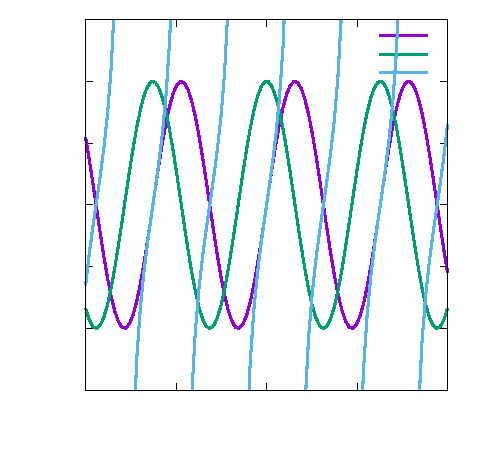
\includegraphics[width={230.00bp},height={216.00bp}]{test}}%
    \gplfronttext
  \end{picture}%
\endgroup

  %figsize is set in image/test.gp 
  \caption[Short caption for Table of Figures]{Illustration of how to
  include a figure (long text, should not go to Table of Figures).}
  \label{fig:test}
\end{figure}

%%%%%%%%%%%%%%%%%%%%%%%%%%%%%%%%%%%%%%%%%%%%%%%%%%
% Keep the following \cleardoublepage at the end of this file, 
% otherwise \includeonly includes empty pages.
\cleardoublepage

% vim: tw=70 nocindent expandtab foldmethod=marker foldmarker={{{}{,}{}}}
